\documentclass{beamer}

\usepackage[T3]{fontenc}
\usepackage[utf8]{inputenc}
\usepackage[russian]{babel}

\usepackage{mhchem}
\usepackage{amssymb, amsmath}

%\usetheme{AnnArbor}
%\usetheme{Antibes}
%\usetheme{Bergen}
\usetheme{Berkeley}
%\usetheme{Berlin}
%\usetheme{Boadilla}
%\usetheme{boxes}
%\usetheme{CambridgeUS}
%\usetheme{Copenhagen}
%\usetheme{Darmstadt}
%\usetheme{default}
%\usetheme{Frankfurt}
%\usetheme{Goettingen}
%\usetheme{Hannover}
%\usetheme{Ilmenau}
%\usetheme{JuanLesPins}
%\usetheme{Luebeck}
%\usetheme{Madrid}
%\usetheme{Malmoe}
%\usetheme{Marburg}
%\usetheme{Montpellier}
%\usetheme{PaloAlto}
%\usetheme{Pittsburgh}
%\usetheme{Rochester}
%\usetheme{Singapore}
%\usetheme{Szeged}
%\usetheme{Warsaw}

\title{Отчет}

\author{Финенко Артем}

\institute[MSU] % (optional, but mostly needed)
{
  МГУ им. М.В.Ломоносова \\
  Химический факультет
}

\date{11/11/2016}

\pgfdeclareimage[height=0.5cm]{university-logo}{../pictures/logo.jpg}
\logo{\pgfuseimage{university-logo}}

\begin{document}

\begin{frame}
  \titlepage
\end{frame}

\begin{frame}{Синтез 2-бензилиденциклопентанона}
\begin{block}{Схема реакции}
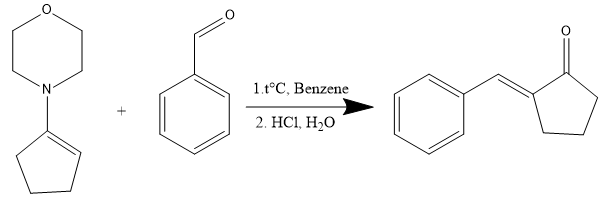
\includegraphics[scale=0.5]{../pictures/1.png}
\end{block}
\begin{block}{}
Выход: 4.8 г (44.75$\%$). \\
Температура плавления: T$_{melt.}$ = 62 - 63$^{\circ}$С, T$_{melt.}^{lit.}$ = 60 - 62$^{\circ}$C \ [1] \\
\end{block}
\end{frame}

\begin{frame}{ЯМР}
\begin{block}{1H-NMR}
\begin{center}
  \makebox[\textwidth]{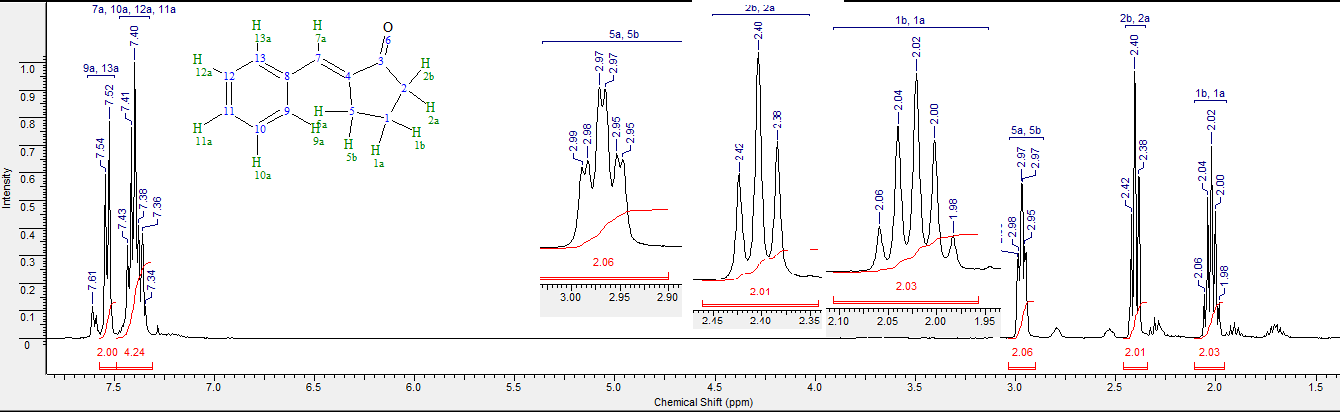
\includegraphics[width=0.8\paperwidth, height=5cm]{../pictures/FAA-K4-02.png}}
\end{center}
\end{block}
\end{frame}

\begin{frame}{Синтез 2-бензилиден-5-(4-метоксибензилиден)циклопентанона.}
\begin{block}{Схема реакции}
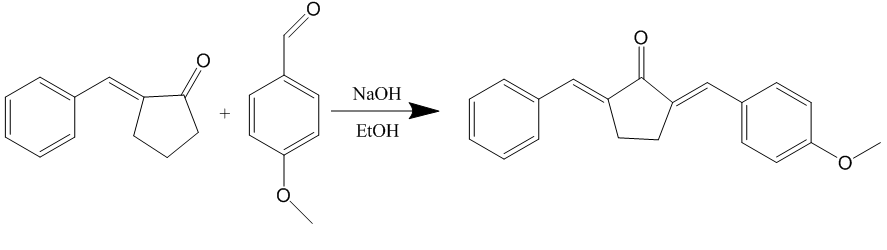
\includegraphics[scale=0.31]{../pictures/2.png}
\end{block}
\begin{block}{}
Выход: 118 мг (40.69$\%$). \\
Температура плавления: T$_{melt.}$ = 169-170$^{\circ}$С, T$_{melt.}^{lit.}$ = 170-171$^{\circ}$C \ [2] \\
\end{block}
\end{frame}

\begin{frame}{ЯМР}
\begin{block}{1H-NMR}
\begin{center}
  \makebox[\textwidth]{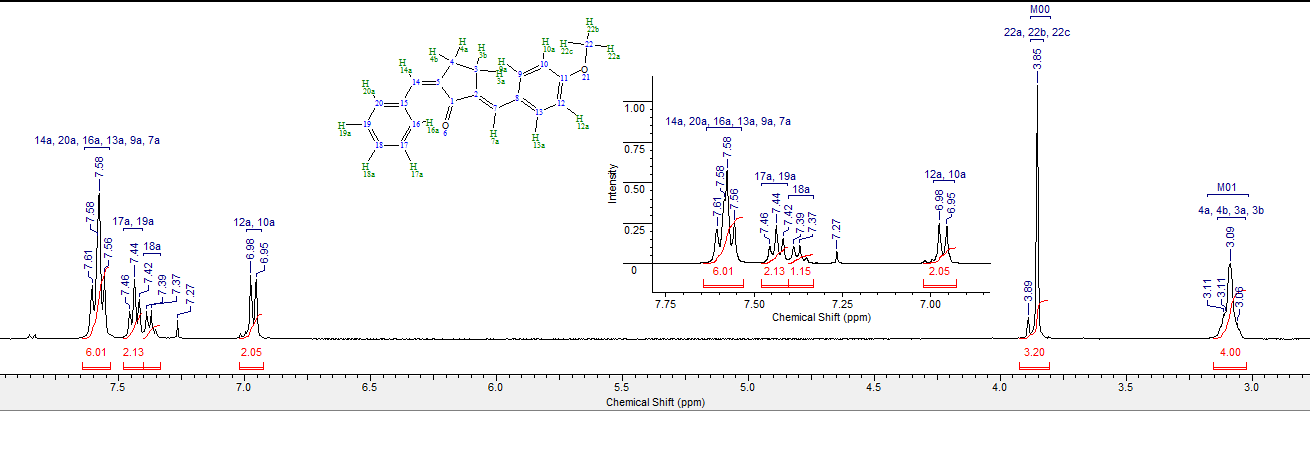
\includegraphics[width=0.8\paperwidth, height = 5cm]{../pictures/FAA-K4-08.png}}
\end{center}
\end{block}
\end{frame}

\begin{frame}{Синтез 2-бензилиден-5-(пиридин-3-илметилен)циклопентанона.}
\begin{block}{Схема реакции}
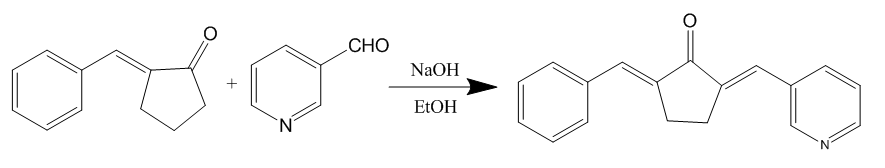
\includegraphics[scale=0.31]{../pictures/3.png}
\end{block}
\begin{block}{}
Выход: 117 мг (44.83$\%$). \\
Температура плавления: T$_{melt.}$ = 187-188$^{\circ}$С, T$_{melt.}^{lit.}$ = 198$^{\circ}$C. \ [3] \\
\end{block}
\end{frame}

\begin{frame}{ЯМР}
\begin{block}{1H-NMR}
\begin{center}
  \makebox[\textwidth]{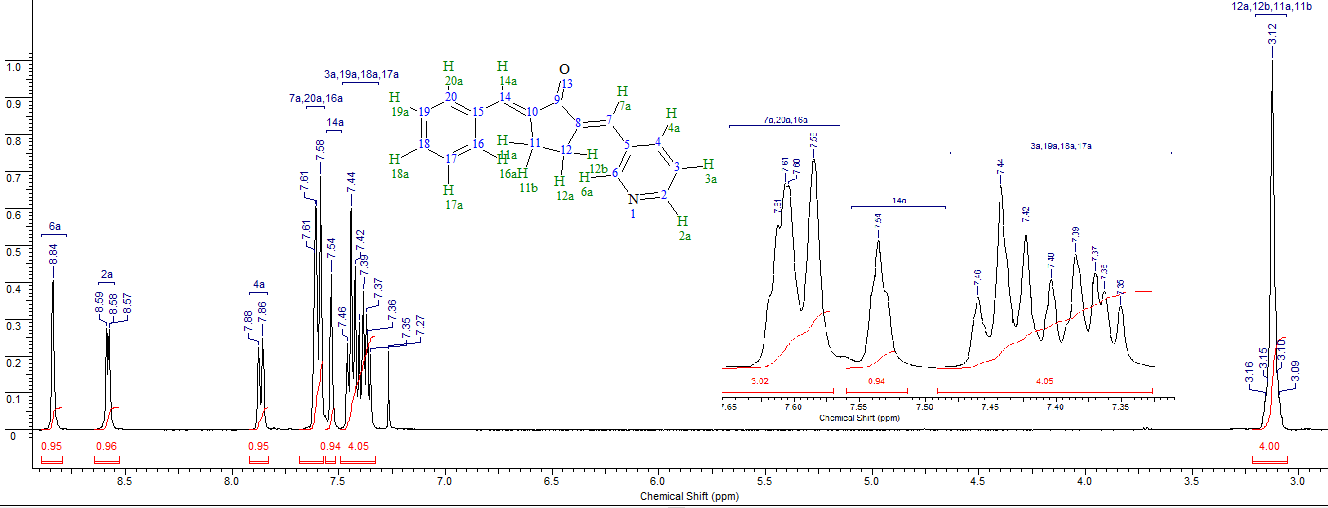
\includegraphics[width=0.8\paperwidth, height = 5cm]{../pictures/FAA-K4-07.png}}
\end{center}
\end{block}
\end{frame}

\begin{frame}{Синтез бензил-1,4-диил-диметилидендициклопентанона.}
\begin{block}{Схема реакции}
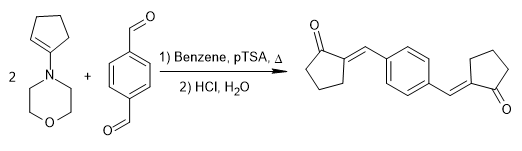
\includegraphics[scale=0.5]{../pictures/4.png}
\end{block}
\begin{block}{}
Выход: 2.32 г (34.89 $\%$). \\
Температура плавления: T$_{melt.}$ = 181-184$^{\circ}$С, T$_{melt.}^{lit.}$ = 185$^{\circ}$C \ [4] \\
\end{block}
\end{frame}

% All of the following is optional and typically not needed. 
\appendix
\section<presentation>*{\appendixname}
\subsection<presentation>*{Bibliography}

\begin{frame}[allowframebreaks]
  \frametitle<presentation>{Bibliography}
    
  \begin{thebibliography}{6}
    
  \beamertemplatebookbibitems
    
  \bibitem{takeishi2004}
    K.~Takeishi, K.~Sugishima.
    \newblock{\em Rhodium-catalyzed intramolecular hydroacylation of 5- and 6-alkynals: Convenient synthesis       of $\alpha$-alkylidenecycloalkanones and cycloalkenones}
    \newblock Chemistry - A European Journal, 2004

  \bibitem{rosamilia2006}
    A.~Rosamilia, M.~Giarusso, J.~Scott, C.~Strauss.
    \newblock{\em  A direct, efficient synthesis of unsymmetrically substituted bis(arylidene)alkanones}
    \newblock Green Chemistry, 2006   

  \bibitem{vatsadze2005}
    S.Z.~Vatsadze, N.~Sviridenkova, M.~Manaenkova, V.~Semashkov, N.~Zyk.
    \newblock{\em Synthesis of unsymmetrical dienones with heteroatomic substituents}
    \newblock Russian Chemical Bulletin, 2005
 
  \bibitem{dimmock2002}
    J.~Dimmock $\textit{et al.}$.
    \newblock{\em Cytotoxic 1,4-bis(2-oxo-1-cycloalkylmethylene)benzenes and related compounds}
    \newblock European Journal of Medicinal Chemistry, 2002 
 
  \end{thebibliography}
\end{frame}

\end{document}